% Architecture of the selective-attention fusion model (lidar_bedlam/models).
% Build: cd .docs/figures && pdflatex architecture.tex
%        pdftoppm -png -r 220 -singlefile architecture.pdf architecture
% Every number comes from the code: models/fusion.py (ModelConfig, SmplHeads,
% translation), models/selective_attention.py (JOINT_GROUPS, gate), models/vit.py
% (VIT_H), models/point_encoder.py (PointTokenizer), losses/smpl.py (LossWeights).
\documentclass[tikz,border=6pt]{standalone}
\usepackage[T1]{fontenc}
\usepackage{lmodern}
\usepackage{helvet}
\usepackage{amsmath}
\renewcommand{\familydefault}{\sfdefault}
\usetikzlibrary{positioning,arrows.meta,fit,backgrounds,calc}

\definecolor{imgfill}{HTML}{E8F0FB}\definecolor{imgline}{HTML}{3F6FB5}
\definecolor{ptsfill}{HTML}{FDEFE2}\definecolor{ptsline}{HTML}{C0722B}
\definecolor{decfill}{HTML}{E9F5F1}\definecolor{decline}{HTML}{1F7A66}
\definecolor{headfill}{HTML}{F5F5F5}\definecolor{headline}{HTML}{4A4A4A}
\definecolor{newfill}{HTML}{FFF6D6}\definecolor{newline}{HTML}{9A7B00}
\definecolor{sub}{HTML}{5B6670}

\tikzset{
  box/.style={draw, line width=0.7pt, rounded corners=3pt, align=center,
              inner sep=6pt, minimum height=11mm, font=\small},
  small/.style={font=\scriptsize\color{sub}},
  img/.style={box, fill=imgfill, draw=imgline, text width=36mm},
  pts/.style={box, fill=ptsfill, draw=ptsline, text width=36mm},
  enc/.style={box, fill=imgfill, draw=imgline, text width=40mm},
  penc/.style={box, fill=ptsfill, draw=ptsline, text width=40mm},
  dec/.style={box, fill=white, draw=decline, text width=34mm},
  head/.style={box, fill=headfill, draw=headline, text width=44mm},
  new/.style={box, fill=newfill, draw=newline, text width=44mm},
  flow/.style={-{Stealth[length=2.4mm]}, line width=0.8pt, draw=black!70},
}

\hyphenpenalty=10000 \exhyphenpenalty=10000
\begin{document}
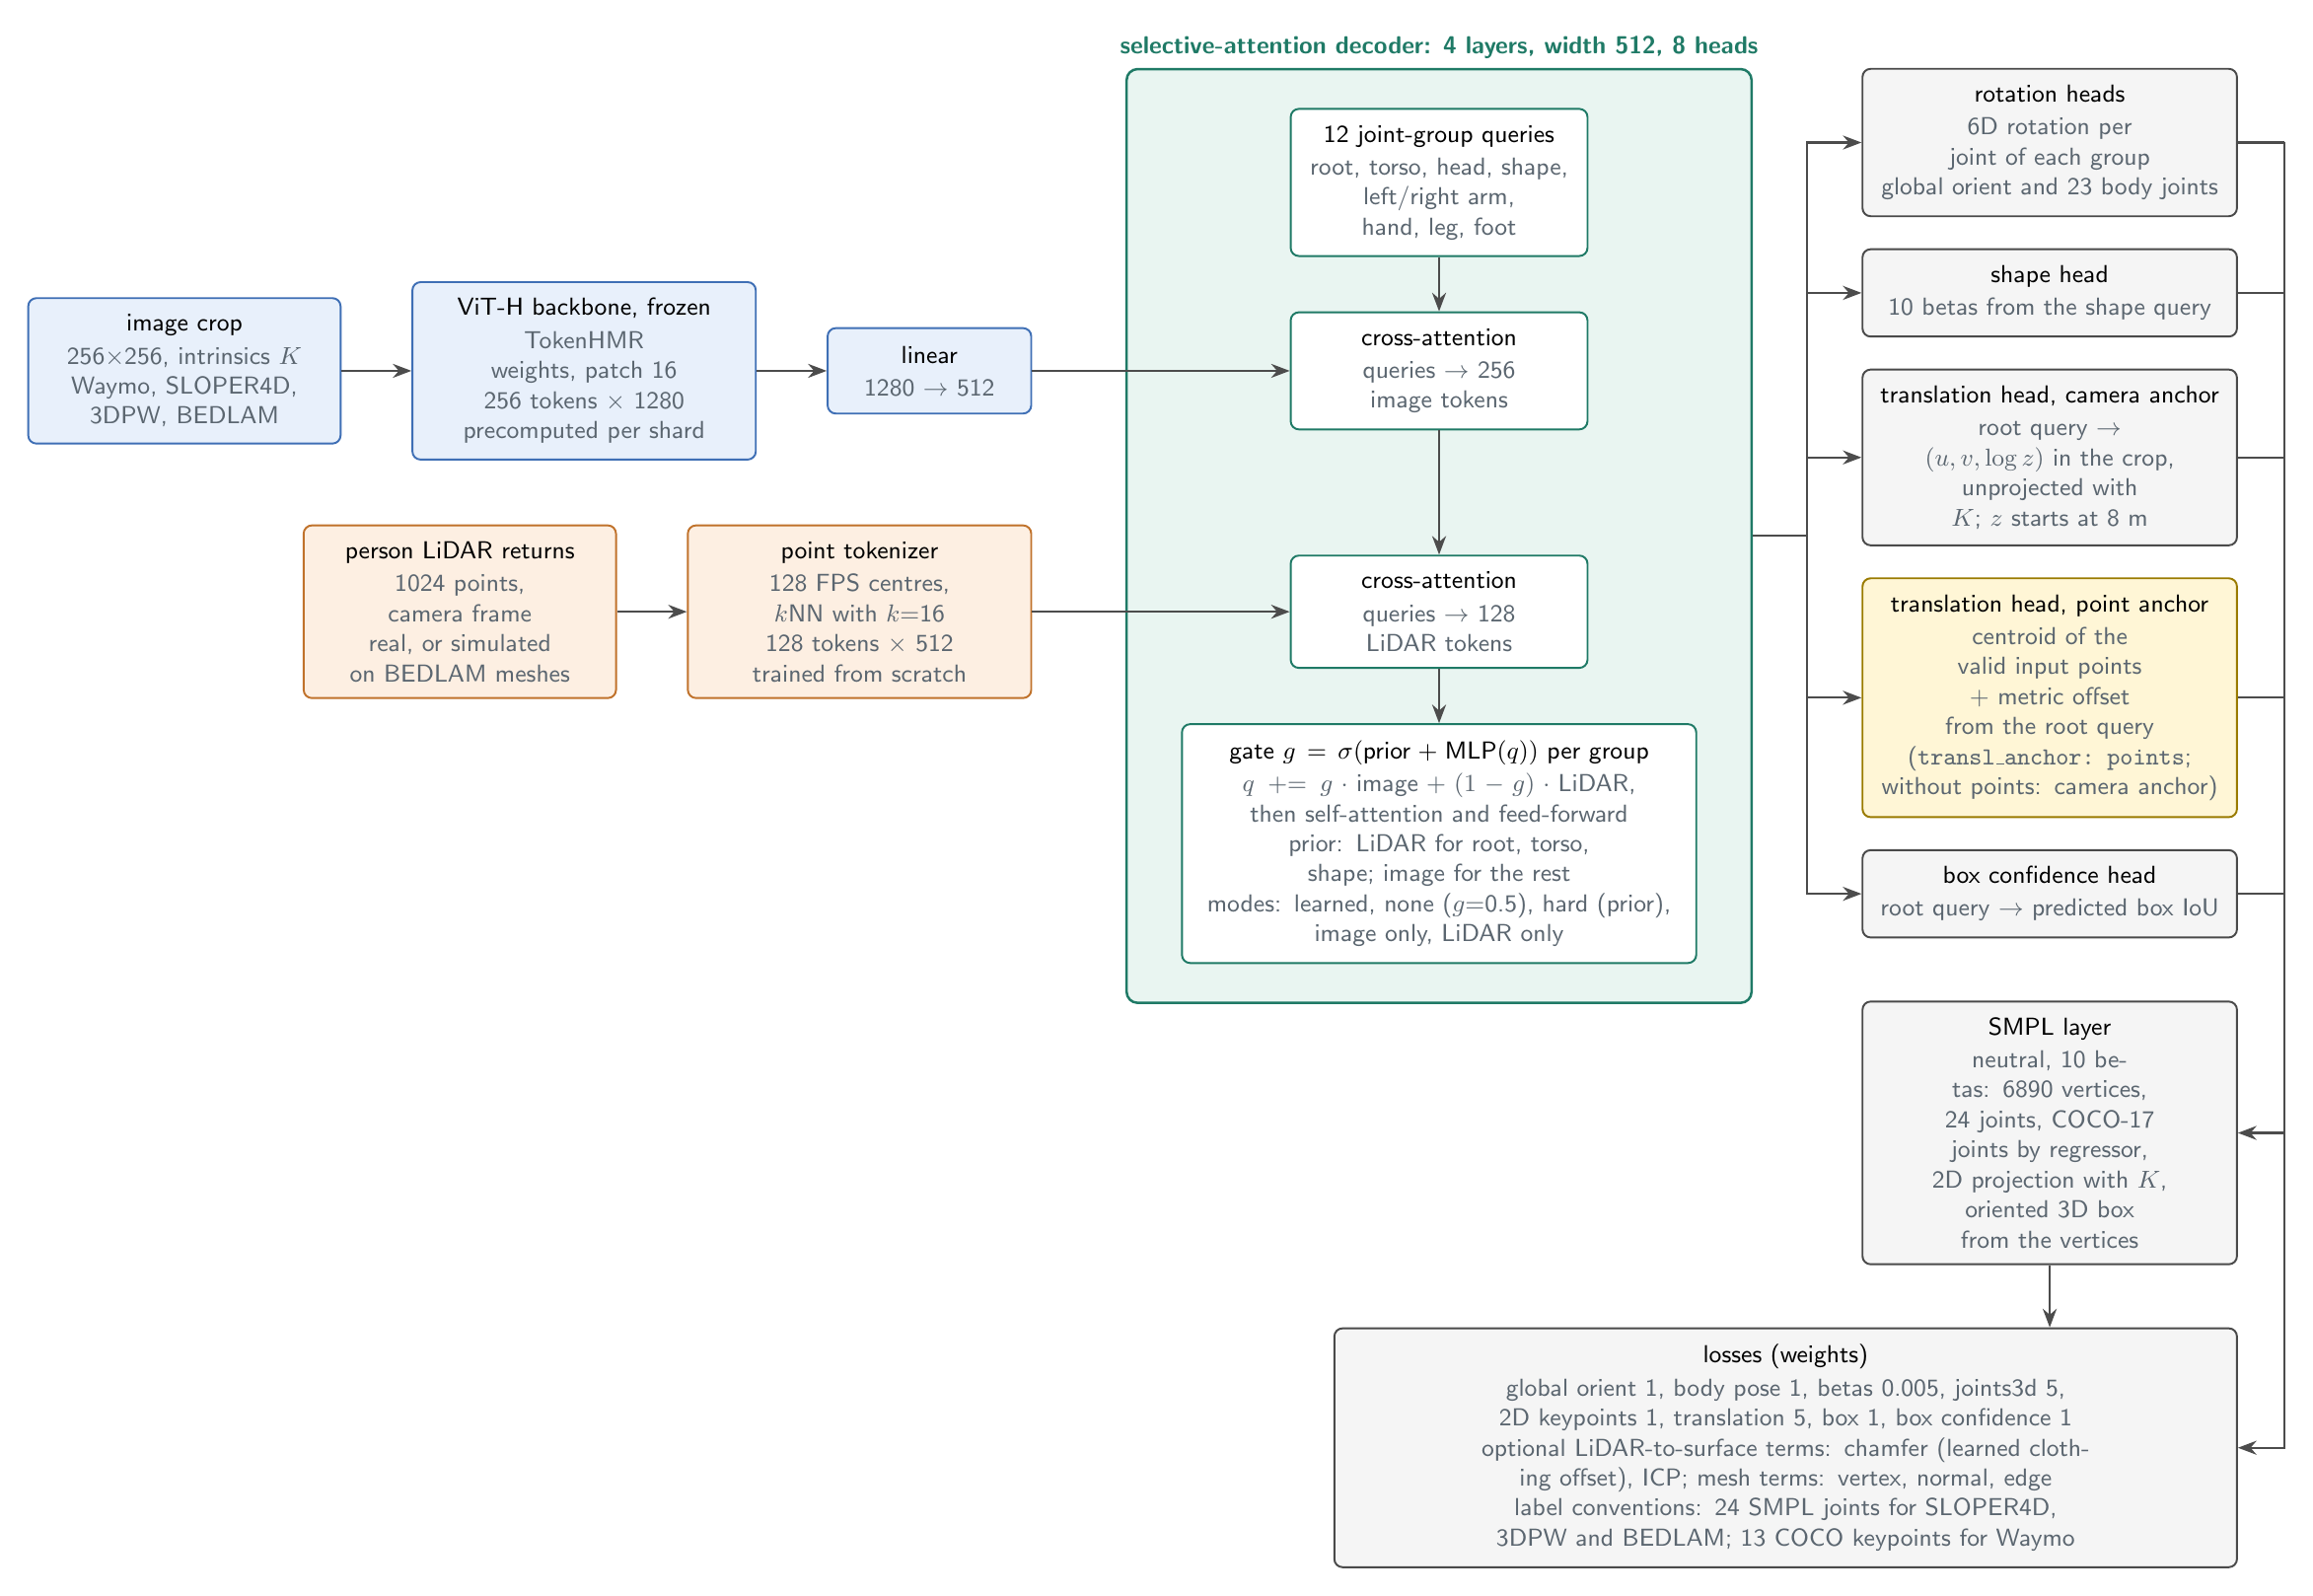
\begin{tikzpicture}[node distance=6mm and 9mm]

% ---- decoder core: image cross-attention on the image row, LiDAR below ----
\node[dec] (xi) {cross-attention\\[1pt]\small\color{sub}queries $\to$ 256 image tokens};
\node[dec, below=16mm of xi] (xp) {cross-attention\\[1pt]\small\color{sub}queries $\to$ 128 LiDAR tokens};
\node[dec, above=7mm of xi] (queries) {12 joint-group queries\\[1pt]
  \small\color{sub}root, torso, head, shape,\\
  \small\color{sub}left/right arm, hand, leg, foot};
\node[dec, below=7mm of xp, text width=62mm] (gate)
  {gate $g=\sigma(\text{prior}+\text{MLP}(q))$ per group\\[1pt]
   \small\color{sub}$q \mathrel{+}= g\cdot\text{image} + (1-g)\cdot\text{LiDAR}$,\\
   \small\color{sub}then self-attention and feed-forward\\
   \small\color{sub}prior: LiDAR for root, torso, shape; image for the rest\\
   \small\color{sub}modes: learned, none ($g$=0.5), hard (prior),\\
   \small\color{sub}image only, LiDAR only};
\begin{scope}[on background layer]
  \node[draw=decline, fill=decfill, rounded corners=4pt, line width=0.9pt,
        fit=(queries)(xi)(xp)(gate), inner xsep=7mm, inner ysep=5mm] (decoder) {};
\end{scope}
\node[font=\small\bfseries\color{decline}, anchor=south] at (decoder.north)
  {selective-attention decoder: 4 layers, width 512, 8 heads};

% ---- image path, on the row of the image cross-attention -----------------
\node[enc, left=12mm of decoder.west |- xi, text width=22mm] (proj) {linear\\[1pt]
  \small\color{sub}1280 $\to$ 512};
\node[enc, left=of proj] (vit) {ViT-H backbone, frozen\\[1pt]
  \small\color{sub}TokenHMR weights, patch 16\\
  \small\color{sub}256 tokens $\times$ 1280\\
  \small\color{sub}precomputed per shard};
\node[img, left=of vit] (crop) {image crop\\[1pt]
  \small\color{sub}256$\times$256, intrinsics $K$\\
  \small\color{sub}Waymo, SLOPER4D,\\
  \small\color{sub}3DPW, BEDLAM};

% ---- point path, on the row of the LiDAR cross-attention -----------------
\node[penc, left=12mm of decoder.west |- xp] (tok) {point tokenizer\\[1pt]
  \small\color{sub}128 FPS centres, $k$NN with $k$=16\\
  \small\color{sub}128 tokens $\times$ 512\\
  \small\color{sub}trained from scratch};
\node[pts, left=of tok] (points) {person LiDAR returns\\[1pt]
  \small\color{sub}1024 points, camera frame\\
  \small\color{sub}real, or simulated\\
  \small\color{sub}on BEDLAM meshes};

% ---- heads, right of the decoder ------------------------------------------
\node[head, anchor=north west] (rot) at ($(decoder.north east)+(14mm,0)$) {rotation heads\\[1pt]
  \small\color{sub}6D rotation per joint of each group\\
  \small\color{sub}global orient and 23 body joints};
\node[head, below=4mm of rot] (shape) {shape head\\[1pt]
  \small\color{sub}10 betas from the shape query};
\node[head, below=4mm of shape] (tcam) {translation head, camera anchor\\[1pt]
  \small\color{sub}root query $\to (u, v, \log z)$ in the crop,\\
  \small\color{sub}unprojected with $K$; $z$ starts at 8 m};
\node[new, below=4mm of tcam] (tpts) {translation head, point anchor\\[1pt]
  \small\color{sub}centroid of the valid input points\\
  \small\color{sub}+ metric offset from the root query\\
  \small\color{sub}(\texttt{transl\_anchor: points};\\
  \small\color{sub}without points: camera anchor)};
\node[head, below=4mm of tpts] (conf) {box confidence head\\[1pt]
  \small\color{sub}root query $\to$ predicted box IoU};

% ---- SMPL under the heads, losses under everything ------------------------
\node[head, below=8mm of conf] (smpl) {SMPL layer\\[1pt]
  \small\color{sub}neutral, 10 betas: 6890 vertices,\\
  \small\color{sub}24 joints, COCO-17 joints by regressor,\\
  \small\color{sub}2D projection with $K$,\\
  \small\color{sub}oriented 3D box from the vertices};
\node[head, text width=112mm, anchor=north east] (loss) at ($(smpl.south east)+(0,-8mm)$) {losses (weights)\\[1pt]
  \small\color{sub}global orient 1, body pose 1, betas 0.005, joints3d 5, 2D keypoints 1, translation 5, box 1, box confidence 1\\
  \small\color{sub}optional LiDAR-to-surface terms: chamfer (learned clothing offset), ICP; mesh terms: vertex, normal, edge\\
  \small\color{sub}label conventions: 24 SMPL joints for SLOPER4D, 3DPW and BEDLAM; 13 COCO keypoints for Waymo};

% ---- arrows ----------------------------------------------------------------
\draw[flow] (crop) -- (vit);
\draw[flow] (vit) -- (proj);
\draw[flow] (proj) -- (xi);
\draw[flow] (points) -- (tok);
\draw[flow] (tok) -- (xp);
\draw[flow] (queries) -- (xi);
\draw[flow] (xi) -- (xp);
\draw[flow] (xp) -- (gate);
% decoder output to every head: one bus
\coordinate (bus) at ($(decoder.east)+(7mm,0)$);
\draw[flow, -] (decoder.east) -- (bus);
\foreach \h in {rot,shape,tcam,tpts,conf} {\draw[flow] (bus) |- (\h.west);}
% heads to the SMPL layer, and the confidence to the loss: a bus on the right
\coordinate (rbus) at ($(conf.east)+(6mm,0)$);
\foreach \h in {rot,shape,tcam,tpts} {\draw[flow, -] (\h.east) -- (\h.east -| rbus);}
\draw[flow] (rot.east -| rbus) -- (smpl.east -| rbus) -- (smpl.east);
\draw[flow] (conf.east) -- (conf.east -| rbus) |- (loss.east);
\draw[flow] (smpl) -- (smpl.south |- loss.north);
\end{tikzpicture}
\end{document}
